\documentclass{sintefposter}

\usepackage{graphicx}
\usepackage{mathtools}
\usepackage{fontspec}
\usepackage{unicode-math}
\defaultfontfeatures{Scale=MatchLowercase}
\usepackage{carlito,tgtermes}
\setmathfont[Ligatures=TeX]{TeX Gyre Termes Math}
\usepackage{microtype}
\usepackage{booktabs}
\usepackage{tikz}
\usepackage{biblatex}
\DeclareSourcemap{
  \maps[datatype=bibtex]{
    \map{
      \step[fieldsource=doi,final]
      \step[fieldset=url,null]
    }  
  }
}

\DefineBibliographyStrings{english}{%
  bibliography = {References},
}


\addbibresource{common/refs.bib}

\tikzstyle{vertex}=[circle, draw, thick]

% Set font to Calibri, or Times clone for serif
\renewcommand{\familydefault}{\sfdefault}



\DeclarePairedDelimiter\ket{\lvert}{\rangle}
\DeclarePairedDelimiter\bra{\langle}{\rvert}
\DeclarePairedDelimiter\p{(}{)}
\DeclarePairedDelimiterX\innerp[2]{\langle}{\rangle}{#1,#2}
\DeclarePairedDelimiterX\braket[3]{\langle}{\rangle}%
  {#1\,\delimsize\vert\,\mathopen{}#2\,\delimsize\vert\,\mathopen{}#3}
\DeclarePairedDelimiter\abs{\lvert}{\rvert}


% just to make sure it exists
\providecommand\given{}
% can be useful to refer to this outside \Set
\NewDocumentCommand\SetSymbol { O{} }{%
  \nonscript\:#1\vert
  \allowbreak
  \nonscript\:
  \mathopen{}
}
\DeclarePairedDelimiterX\Set[1]\{\}{%
  \renewcommand\given{\SetSymbol[\delimsize]}
  #1
}

\DeclareMathOperator\dd{d}
\DeclareMathOperator{\cnot}{\symtt{CNOT}}
\DeclareMathOperator{\cz}{\symtt{CZ}}
\DeclareMathOperator{\id}{I}
\newcommand{\paulix}{{\sigma_x}}
\newcommand{\pauliy}{{\sigma_y}}
\newcommand{\pauliz}{{\sigma_z}}


\newcommand\spaceScript[1]{\ensuremath{\scriptscriptstyle(#1)}}

\title{Measurement-Based Quantum Computing}
\author{Utku Birkan\\ Advisor: Sadi Turgut}
\institute{Department of Physics, ODTÜ}


\begin{document}
\maketitle

% Tip: for long titles, use \parbox{\linewidth}{text}


\begin{columns}
\column{0.5}

\block{Abstract}{
  In this prjoect we insvestigate measurement-based quantum computing (MBQA), a novel approach to quantum computing which uses projective measurements to achieve universal computation instad of using unitary evolution. Through this project, we introduce the concept of graph states, then formulate an abstract machine on top of this construct. We then provide a prood of universality, and the demonstrate MBQA through a toy problem, Deutsch algorithm. 
}


\block{Method}{
  The main structure used by measurement-based quantum compuitng is a \emph{graph state}\cite{hein2006}. Graph states are multi qubit systems which can be described by a simple graph. For a graph \(G=\Set{V, E}\), its graph state is defined by the following set of commutative, Hermitian operators it is stabilized by.
  \begin{equation}
    K=\Set*{K_a = \sigma_x^a\prod_{b\in N_a} \sigma_z^b \given a \in V },
  \end{equation}
  where \(N_a\) is the neighborhood of vertex \(a\). Such a graph state can be generated via the following procedure.
  \begin{enumerate}
    \item For each vertex in \(V\), initialize the corresponding qubit with the positive \(\sigma_x\) eigenstate \(\ket+\).
    \item For each edge \(\p{a,b}\in E\), apply the conditonal phase flip gate \(S_{ab} = \ket0\bra0\otimes\symbb1 + \ket1\bra1\otimes\sigma_z\) to the system.
  \end{enumerate}\vspace{\baselineskip}
  
  An abstract machine, \textcolor{red}{one-way quantum computer}\cite{russendorf2003}, can be constructed with a \emph{cluster}, a graph state with a regular lattice structure that acts a substrate to perform computations, and a \emph{random access measurement device} to measure the qubits in the cluster. The computer takes a measurement pattern
  \begin{equation}
    \symcal{M} = \Set{\vec{r}_a \given a \in V},
  \end{equation}
  composed of a measurement direction for each qubit, as its input program.\vspace{\baselineskip}

  Circuit-based computers use deterministic unitary evolution for program evolution while one-way computers use probabilistic projective measurements. Even then, these two have the same computational power. This fact can be directly proven by providing a mechanism to simulate unitary evolution using the one-way computer. \vspace{\baselineskip}

  One-way computer can simulate a unitary \(U\) up to some Pauli element called the \emph{by-product operator \(U_\Sigma\)}\cite{russendorf2003} that is parameterized by previous measurement outcomes.
  \begin{equation}
    U' = U_\Sigma\,U \quad \text{is simulated.}
  \end{equation}
  Note that since measurement outcomes are classical data, byproduct operators can be handled by the computer's controller via adapting the next measurement basis during program execution. Any unitary unitary circuit can be rewritten using the universal gates \(\cnot\) and arbitrary single-qubit rotation \(R(\alpha, \beta, \gamma)\)\cite{Nielsen2009}. These two can be implemented by the following operations. \(R(\alpha, \beta, \gamma) = R_x(\alpha) R_y(\beta) R_z(\gamma)\) is an Euler rotation. Let
  \begin{equation}
    \symcal{B}(\varphi) = \Set*{\frac{\ket0 + e^{i\varphi}\ket1}{\sqrt2}, \frac{\ket0 - e^{i\varphi}\ket1}{\sqrt2}}
  \end{equation}
  be a parameterized projection basis. Measuring a 4-qubit linear cluster in the basis \(\symcal{B}(\alpha)\), \(\symcal{B}((-1)^{s_1}\beta)\) and \(\symcal{B}((-1)^{s_2}\gamma)\) implements 
  \begin{equation}
    \underbrace{\sigma_x^{s_2+s_4}\sigma_z^{s_1+s_3}}_{U_\Sigma}R(\alpha, \beta, \gamma).
  \end{equation} 
}




\column{0.5}

\block{}{
  \vspace*{-\baselineskip}
  For \(\cnot\), we use the graph state below which implementes \(\sigma_{x,\text{out}}^{s_2} \sigma_{z,\text{out}}^{s_1} \sigma_{z,\text{ctrl}}^{s_2} \cnot\) where filled nodes are measured on \(\sigma_x\) basis.
  \begin{center}
    \scalebox{0.6}{
    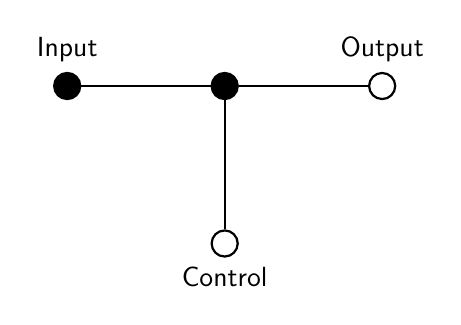
\begin{tikzpicture}[transform shape]
      \node[vertex, fill, label=above:Input](v1) at (0, 0) {};
      \node[vertex, fill](v2) at (2, 0) {};
      \node[vertex, label=above:Output](v3) at (4, 0) {};
      \node[vertex, label=below:Control](v4) at (2,-2) {};            
      \begin{scope}[every path/.style={-, thick}]
        \draw (v1) -- (v2);
        \draw (v2) -- (v3);
        \draw (v2) -- (v4);
      \end{scope} 
    \end{tikzpicture}}
  \end{center}
  
  Lastly, we introduce two useful identities. Firstly, measuring a qubit in \(\sigma_z\) basis effectively removes it from the cluster with a by-product \(\sigma_x^s\). Secondly, measuring a qubit in \(\sigma_x\) in a wire teleports its state to the next vertex.
}
\block{Results}{
  This project had two phases. The first phase involves the theoretical investigation of measurement-based quantum computing (MBQC). During this phase we reviewed graph states, stabilizer formalism. Furthermore, we introduced the one-way quantum computer as an abstract machine and given a constructive proof of the universality of MBQC, whcih is a fundamental property.\vspace{\baselineskip}

  Next, we survayed various simulators to test this framework as there are no real quantum computing backends utilizing MBQC that are available to public use. At the time of writing, there are two alternative simulators. Open sourced \texttt{quantumcore}\cite{quantumCore} library, which was reported to be used for simulating Deutsch-Jozsa algorithm using MBQC, lacks a public driver and lack any kind of documentation so we were not able to utilize it. The other alternative is a new addition to \texttt{pebble quantum}\cite{Paddlequantum}, a quantum machine learning platform. Even though we were not able to successfully test a multi-bit function types via Deutsch-Jozsa algorithm, we were able to test single-bit functions using the simpler Deutsch algorithm. Oracle implementations and simulation outcomes are given in Table 1.
  \begin{center}
    \begin{tabular}{lrlr}
      \toprule
      Function & Implementation & Type &  Outcome \\
      \midrule 
      $f(x) = 0$ & $\symbb1$ & Constant & $0$ \\
      $f(x) = 1$ & $\sigma_x^{\scriptsize(0)} $ & Constant & $0$\\
      $f(x) = x$ & $CX$ & Balanced & $1$\\
      $f(x) = \neg x$ & $\sigma_x^{\scriptsize(0)} CX$ & Balanced & $1$ \\
      \bottomrule
    \end{tabular}\vspace{4pt}
    
    \textbf{Table 1:} Function Implementations Used for Deutsch Oracles 
  \end{center}
}


\block{References}{
  \printbibliography[heading=none]
}


\end{columns}


\end{document}

